%%%%%%%%%%%%%%%%%%%%%%%%%%%%%%%%%%%%%%%%%%%%%%%%%%%%%%%%%%%%%%%%%%%%%%%%%%%%%%%%%%
\begin{frame}[fragile]\frametitle{}
\begin{center}
{\Large  Deep Learning from Scratch using Python}
\end{center}
{\tiny (How to build a simple neural network in 9 lines of Python code - Milo Spencer-Harper)}
\end{frame}


%%%%%%%%%%%%%%%%%%%%%%%%%%%%%%%%%%%%%%%%%%%%%%%%%%%%%%%%%%%%%%%%%%%%%%%%%%%%%%%%%%
\begin{frame}[fragile]\frametitle{The Program}
\begin{lstlisting}
from numpy import exp, array, random, dot
training_set_inputs = array([[0, 0, 1], [1, 1, 1], [1, 0, 1], [0, 1, 1]])
training_set_outputs = array([[0, 1, 1, 0]]).T
random.seed(1)
synaptic_weights = 2 * random.random((3, 1)) - 1
for iteration in xrange(10000):
    output = 1 / (1 + exp(-(dot(training_set_inputs, synaptic_weights))))
    synaptic_weights += dot(training_set_inputs.T, (training_set_outputs - output) * output * (1 - output))
print 1 / (1 + exp(-(dot(array([1, 0, 0]), synaptic_weights))))
\end{lstlisting}
\end{frame}

%%%%%%%%%%%%%%%%%%%%%%%%%%%%%%%%%%%%%%%%%%%%%%%%%%%
\begin{frame}[fragile] \frametitle{Deep Learning == Neural Network}

\begin{itemize}
\item We model transormation of inputs to outputs using Neural Network
\item We parameters in form of matrices, called weights
\item A large positive weight or a large negative weight, will have a strong effect on the neuron's output.
\item Weigted sum goes through activation function to compute output
\item Diff bwteen computed and actual is the error
\item Error is minimzed by backproggram by adjusting weights. 
\end{itemize}
\end{frame}

%%%%%%%%%%%%%%%%%%%%%%%%%%%%%%%%%%%%%%%%%%%%%%%%%%%%%%%%%%%%%%%%%%%%%%%%%%%%%%%%%%
\begin{frame}[fragile]\frametitle{The Problem}
\begin{center}
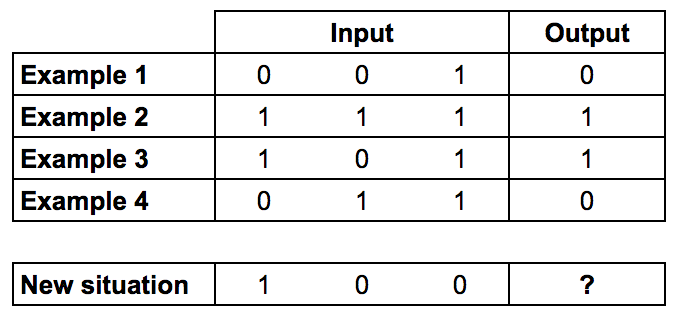
\includegraphics[width=\linewidth,keepaspectratio]{dls1}
\end{center}
You might have noticed, that the output is always equal to the value of the leftmost input column. Therefore the answer is the `?' should be 1.
\end{frame}

%%%%%%%%%%%%%%%%%%%%%%%%%%%%%%%%%%%%%%%%%%%%%%%%%%%
\begin{frame}[fragile] \frametitle{Training process}

\begin{itemize}
\item Each input ($x_i$) is given a weight ($w_i$)
\item Weighted sum $\sum w_i . x_i = w_1 . x_1 + w_2 . x_2 + w_2 . x_2$
\item Normalize the result by Sigmoid function so the result is between 0 and 1 
\item $\bar{y} = \frac{1}{1 + e^{-(\sum w_i . x_i )}}$
\item Error $E(w_i) = \bar{y} - y$ 
\item Back Propogation: Adjusting weights $w_i = w_i - \alpha dE/dw$
\item We can simplistically take Adjusting weights, here, as $E.x.y.(1 - y)$ instead of $\alpha dE/dw$ (Approximation, for simplification)
\end{itemize}
\end{frame}

%%%%%%%%%%%%%%%%%%%%%%%%%%%%%%%%%%%%%%%%%%%%%%%%%%%
\begin{frame}[fragile] \frametitle{Constructing the Python code}
Imports and the input-output Training set
\begin{lstlisting}
from numpy import exp, array, random, dot

training_set_inputs = array([[0, 0, 1], [1, 1, 1], [1, 0, 1], [0, 1, 1]])
training_set_outputs = array([[0, 1, 1, 0]]).T
\end{lstlisting}
The `.T' function, transposes the matrix from horizontal to vertical. So the computer is storing the vertical numbershorizontally!!.
\end{frame}

%%%%%%%%%%%%%%%%%%%%%%%%%%%%%%%%%%%%%%%%%%%%%%%%%%%
\begin{frame}[fragile] \frametitle{Constructing the Python code}
\begin{itemize}
\item We model a single neuron, with 3 input connections and 1 output connection.
\item We assign random weights to a 3 x 1 matrix, with values in the range -1 to 1 and mean 0.
\end{itemize}
\begin{lstlisting}
self.synaptic_weights = 2 * random.random((3, 1)) - 1
\end{lstlisting}
\end{frame}

%%%%%%%%%%%%%%%%%%%%%%%%%%%%%%%%%%%%%%%%%%%%%%%%%%%
\begin{frame}[fragile] \frametitle{Constructing the Python code}
Iteration loop
\begin{lstlisting}
for iteration in xrange(10000):
    output = 1 / (1 + exp(-(dot(training_set_inputs, synaptic_weights))))
    synaptic_weights += dot(training_set_inputs.T, (training_set_outputs - output) * output * (1 - output))
\end{lstlisting}
Weights are settled now.
\end{frame}

%%%%%%%%%%%%%%%%%%%%%%%%%%%%%%%%%%%%%%%%%%%%%%%%%%%
\begin{frame}[fragile] \frametitle{Constructing the Python code}
Prediction of unknown
\begin{lstlisting}
print(1 / (1 + exp(-(dot(array([1, 0, 0]), synaptic_weights)))))
\end{lstlisting}
That's it!!
{\tiny (Code available here : https://github.com/miloharper/simple-neural-network)}
\end{frame}